\documentclass[a4paper,12pt,preview]{report} %размер бумаги устанавливаем А4, шрифт 12пунктов
\usepackage[english,russian]{babel}%используем русский и английский языки с переносами 	
\usepackage[T2A]{fontenc}
\usepackage{changepage}
\usepackage{lipsum}
\usepackage{indentfirst}
\usepackage{hyperref}
\usepackage[labelsep=period]{caption}
\usepackage{amsmath}
\usepackage{textcomp}
\usepackage[utf8]{inputenc}%включаем свою кодировку: koi8-r или utf8 в UNIX, cp1251 в Windows
\usepackage[english,russian]{babel}%используем русский и английский языки с переносами 	
\usepackage{amssymb,amsfonts,amsmath,mathtext,cite,enumerate,float} %подключаем нужные пакеты расширений
\usepackage{graphicx} %хотим вставлять в диплом рисунки?
\usepackage{ragged2e}
\usepackage{indentfirst}
\usepackage{titlesec}
\usepackage{listings}
\usepackage{multirow}
\lstset{
	basicstyle=\small\ttfamily,
	columns=flexible,
	breaklines=true
}
\graphicspath{{images/}}%п\usepackage{trd}уть к рисункам

\makeatletter
\renewcommand{\@biblabel}[1]{#1.} % Заменяем библиографию с квадратных скобок на точку:
\makeatother

\usepackage{geometry} % Меняем поля страницы
\geometry{left=2cm}% левое поле
\geometry{right=1.5cm}% правое поле
\geometry{top=1cm}% верхнее поле
\geometry{bottom=2cm}% нижнее поле
\usepackage{hyperref}
\hypersetup{
	colorlinks,
	citecolor=black,
	filecolor=black,
	linkcolor=black,
	urlcolor=black
}

\renewcommand{\theenumi}{\arabic{enumi}}% Меняем везде перечисления на цифра.цифра
\renewcommand{\labelenumi}{\arabic{enumi}}% Меняем везде перечисления на цифра.цифра
\renewcommand{\theenumii}{.\arabic{enumii}}% Меняем везде перечисления на цифра.цифра
\renewcommand{\labelenumii}{\arabic{enumi}.\arabic{enumii}.}% Меняем везде перечисления на цифра.цифра
\renewcommand{\theenumiii}{.\arabic{enumiii}}% Меняем везде перечисления на цифра.цифра
\renewcommand{\labelenumiii}{\arabic{enumi}.\arabic{enumii}.\arabic{enumiii}.}% Меняем везде перечисления на цифра.цифра

\newcommand{\doublerule}[1][.4pt]{%
	\noindent
	\makebox[0pt][l]{\rule[.7ex]{\linewidth}{#1}}%
	\rule[.3ex]{\linewidth}{#1}}



\titleformat{\chapter}[hang]
{\normalfont\huge\bfseries}{\thechapter.}{20pt}{}

%\renewcommand*\thesection{\arabic{section}}

\begin{document}
	
	\begin{center}
		Министерство образования и науки РФ \\
		Федеральное государственное автономное образовательное учреждение высшего профессионального образования <<НИТУ МИСиС>>\\
		Институт ИТАСУ\\
		Кафедра Инженерной кибернетики\\
	\end{center}
	
	
	\vfill
	
	\begin{center}
		\Large\textbf{Курсовая работа \\
			по курсу <<Методы Обработки Изображений>> \\
			на тему: <<Легковесный детектор элементов рекламы>>}
	\end{center}
	
	\vfill
	
	\begin{FlushRight}
		Выполнил\\
		Студент группы \\
		БПМ-16-2 \\
		Фадеев А.Ю. \\
		[\baselineskip]
		Проверил: \\
		доц., к.т.н. Полевой Д.В. \\
		[9\baselineskip]
	\end{FlushRight}
	
	
	\begin{center}
		Москва 2020
	\end{center}
	
	\thispagestyle{empty}
	\newpage
	
	\tableofcontents
	\newpage
	
	
	\chapter{Введение}
	
	В данный момент на большом количестве веб-страницах основным способом монетизации является рекламный контент. Множество сайтов злоупотребляют использованием вставок,
	размещая их в большом количестве и/или размещая отвлекающие вставки. Из вышесказанного следует, что задача обнаружения и скрытия рекламного контента является актуальной.
	Цель этой работы состоит в разработке программного модуля для поиска приблизительного положения таких вставок на изображении.
	
	\chapter{Основная часть}
	
	\section{Введенные обозначения}
	
	
	Введем несколько обозначений:
	
	\begin{itemize}
		\item Обозначим текущий выбранный элемент рекламы за $E$
		\item Обозначим текущий выбранное изображение за $S$
		\item Обозначим множество особых точек на $E$, которые с чем-либо "сматчены" за $pts_E$, а на $S$ -- за $pts_S$.
		\item Обозначим центр масс множества $pts_E$ за $cent_E$, а центр масс $pts_S$ -- за $cent_S$.
		\item Общее количество элементов рекламы обозначим за $cnt_{ads}$
		\item Количество обнаруженных элементов рекламы обозначим за $cnt_{discovered}$
		\item Количество корректных матчингов, которые нашли не элемент рекламы, обозначим за $cnt_{wrong}$
		\item Количество корректных матчингов обозначим за $cnt_{match}$
	\end{itemize}
	
	\section{Формат входных и выходных данных}
	
	В директории ads:
	
	\begin{center}
	\begin{tabular}{| c | c |}
		\hline
		Поддиректория & Что хранит\\		
		\hline
		pages & Исходные изображения.\\
		\hline
		md\_pages & Изображения с размеченными на них документами.\\
		\hline
		\multirow{2}{*}{elements} & Элементы рекламы -- кусочки изображений, \\
		\text{} &  по которым можно определить нахождение рекламы на изображении. \\
		\hline
		\multirow{2}{*}{markdown} & находятся текстовые файлы, \\
		\text{} & в которых содержится информация о разметке. \\
		\hline
		\multirow{2}{*}{result} & результат -- изображения с обозначенными на них распознанными\\
		\text{} & элементами рекламы, а также в statistics.txt \\
		\hline
	\end{tabular}
	\end{center}
	
	
	
	Формат данных в файлах поддиректории markdown:
	
	\begin{itemize}
		\item В первой строке число $n$ - количество прямоугольников.
		\item В следующих $n$ строках -- информация о прямоугольниках. 
		\item В очередной строке находятся 4 числа: координаты $x$, $y$ прямоугольника, ширина и высота прямоугольника. 
	\end{itemize}

	Для того, чтобы изменить место, откуда будут считываться данные, необходимо поменять в файлах \texttt{main\_app.cpp} и \texttt{main\_md.cpp} переменную \texttt{dir\_path}.
	
	
	\section{Методика оценки качества решения}
	
	Критериями качества выбраны 2 характеристики:
	\begin{itemize}
		\item Доля обнаруженных элементов рекламы $= \frac{cnt_{discovered}}{cnt_{ads}}$.
		\item Доля неверных "матчингов" $= \frac{cnt_{wrong}}{cnt_{match}}$.
	\end{itemize}
	



\section{Сборка}

Проект собирается через CMake. Требуется иметь библиотеку OpenCV. Возможно, придется "докидывать" файлы \texttt{.dll} библиотеки в директорию с проектом, либо прописывать путь до них в \textbf{PATH}.

	
	
	\section{Разметка}
	Исходные изображения размечаются вручную.
	
	Например, на изображении
	
	\begin{figure}[H]
		\centering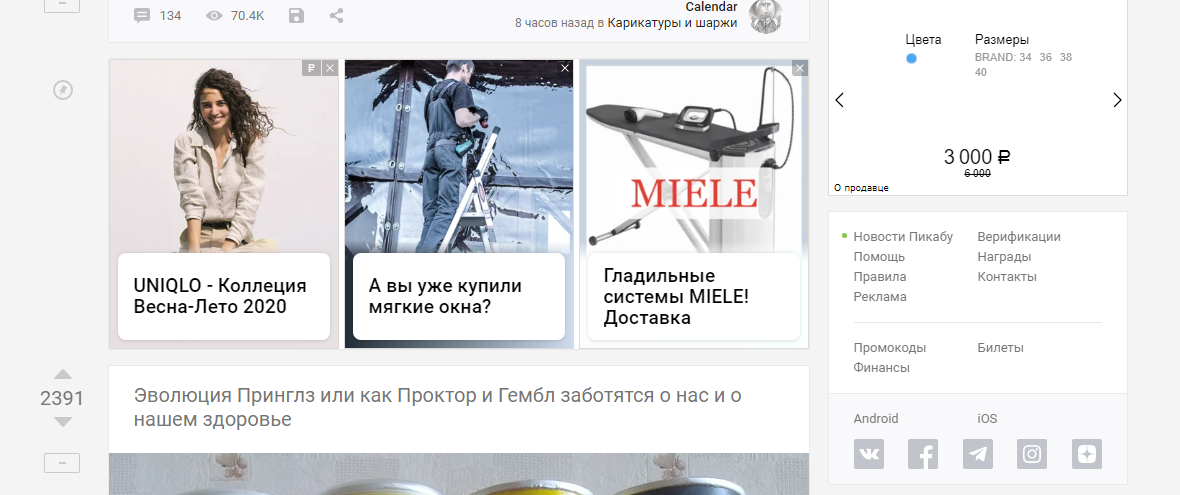
\includegraphics[scale=0.4]{page1.PNG}
		\caption{Исходное изображение}
		\label{fig:page1}
	\end{figure}

	Можно выделить такие элементы рекламы:
	
	\begin{figure}[H]
		\centering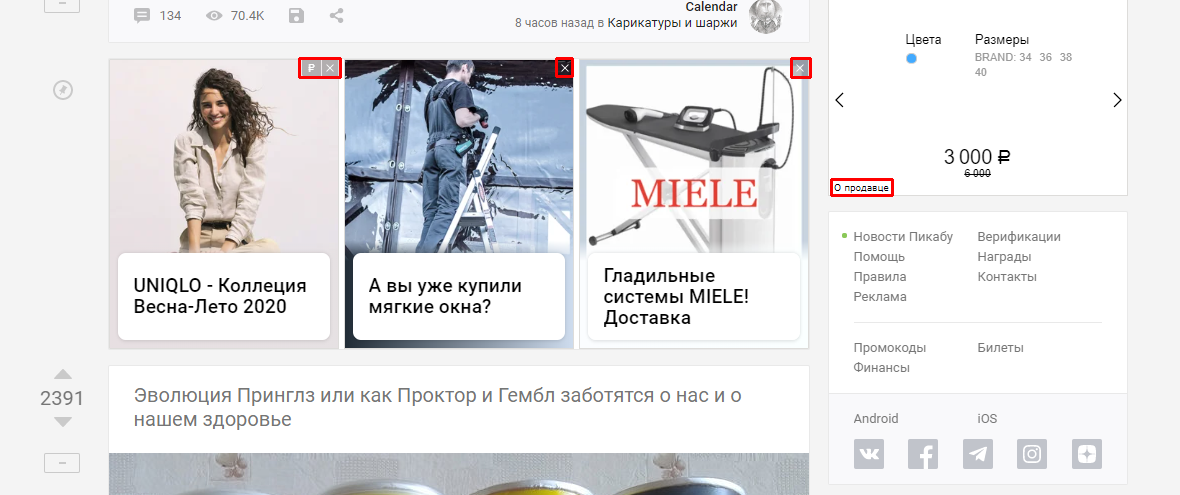
\includegraphics[scale=0.4]{md1.PNG}
		\caption{Размеченное изображение}
		\label{fig:md1}
	\end{figure}
	
	Информация о этих элементах сохраняется, в текстовом виде (информация о прямоугольниках на изображении):
	
	\begin{figure}[H]
		\centering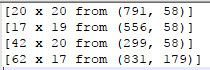
\includegraphics[scale=1.5]{rects1.PNG}
		\caption{Прямоугольники}
		\label{fig:rects1}
	\end{figure}
	
	А также в виде фрагментов изображения:
	
	\begin{figure}[H]
		\centering
\includegraphics[scale=1.5]{el1.PNG}\text{ }
		\centering
\includegraphics[scale=1.5]{el2.PNG}\text{ }
		\centering
\includegraphics[scale=1.5]{el3.PNG}\text{ }
		\centering
\includegraphics[scale=1.5]{el4.PNG}\text{ }
		\caption{Элементы}
		\label{fig:ele1}
	\end{figure}
	
	Для этого используется программа из Приложения А.


	
	\section{Описание алгоритма}
	
	Исходные изображения и все элементы рекламы проходят через SIFT, который ищет в них особые точки.
	
	Примеры:
	
	\begin{figure}[H]
		\centering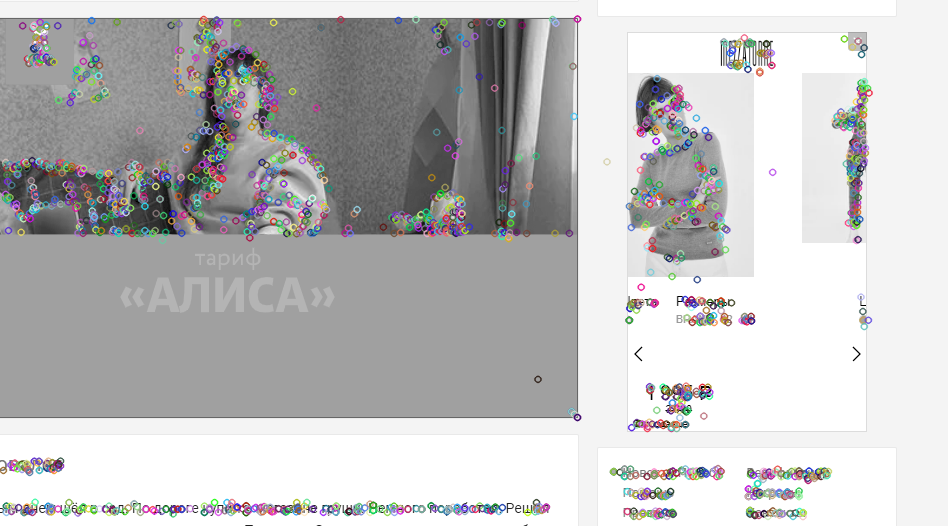
\includegraphics[scale=0.5]{page2.PNG}
		\caption{Особые точки на изображении}
		\label{fig:page2}
	\end{figure}
	
	\begin{figure}[H]
		\centering
\includegraphics[scale=2]{elemmmm.PNG}
		\caption{Особые точки на элементе рекламы}
		\label{fig:elemmmm}
	\end{figure}
	
	
	
	Матчинг производится с помощью алгоритма FLANN.
	
	Далее матчинги проходят проверку на корректность.
	
	
	Проверка на корректность состоит из нескольких этапов:
	\begin{enumerate}
		\item Хотя бы $P\%$ особых точек $E$ должны быть "смэтчены" с какой-либо особой точной на $S$ (в данной работе $P = 75$).
		
		\item Элемент $E$, если и присутствует на $S$, то увеличен не более, чем в $K$ раз (в данной работе $K = 3$).
		
		Математически, это выглядит так:
		
		\begin{equation}
			K \times \rho(pts_{Ei}, cent_E) \geq \rho(pts_{Si}, cent_S), \forall i
		\end{equation}
		
		\item  Углы поменялись не слишком сильно:
		
		\begin{equation}
		angle((pts_{Ei} - cent_E), (pts_{Si} - cent_S)) \leq \varepsilon, \forall i
		\end{equation}
		
		В данной работе $\varepsilon = \pi / 2$.
		
	\end{enumerate}

	Если матчинг выполняет все 3 условия, то он считается корректным. При этом, если $cent_page$ попал внутрь какого-либо элемента рекламы, то этот элемент считается обнаруженным. В обратном случае -- увеличивается $cnt_{wrong}$.
	
	
	\begin{figure}[H]
		\centering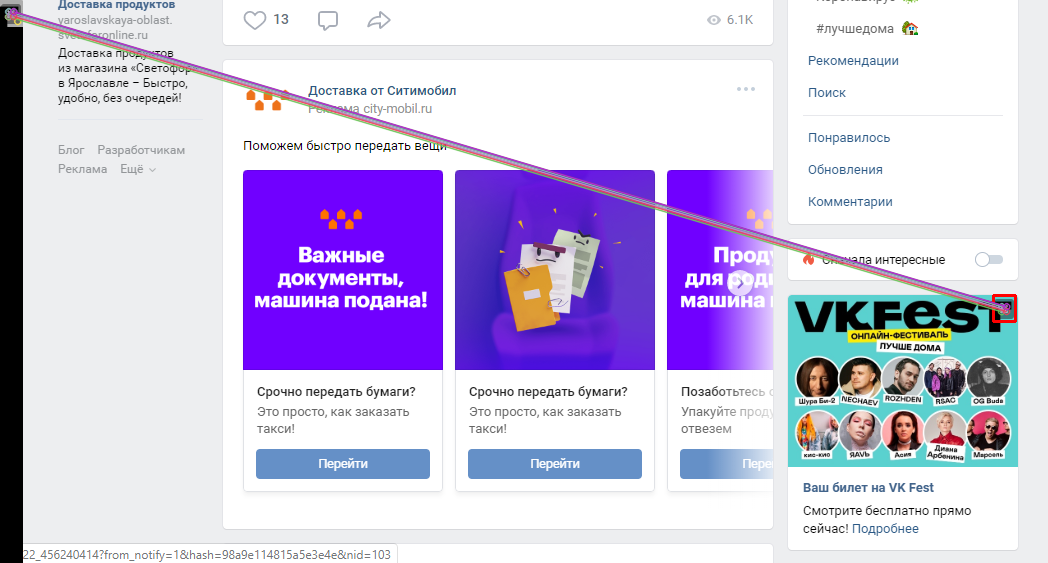
\includegraphics[scale=0.5]{correct_matching.PNG}
		\caption{Пример правильного корректного матчинга}
		\label{fig:correct_matching}
	\end{figure}
	

\section{Результаты}

Итоговая статистика для сгенерированной выборки, она находится в файле statistics.txt.

\begin{itemize}
	\item Количество найденных элементов -- \texttt{12/15}.
	\item Количество неправильных матчингов (которые привели не в элемент рекламы) -- \texttt{0/17}.
\end{itemize}


Пример обработанного изображения, который сохраняется в поддиректорию result. Фиолетовыми кругами отмечены обнаруженные элементы.

	\begin{figure}[H]
		\centering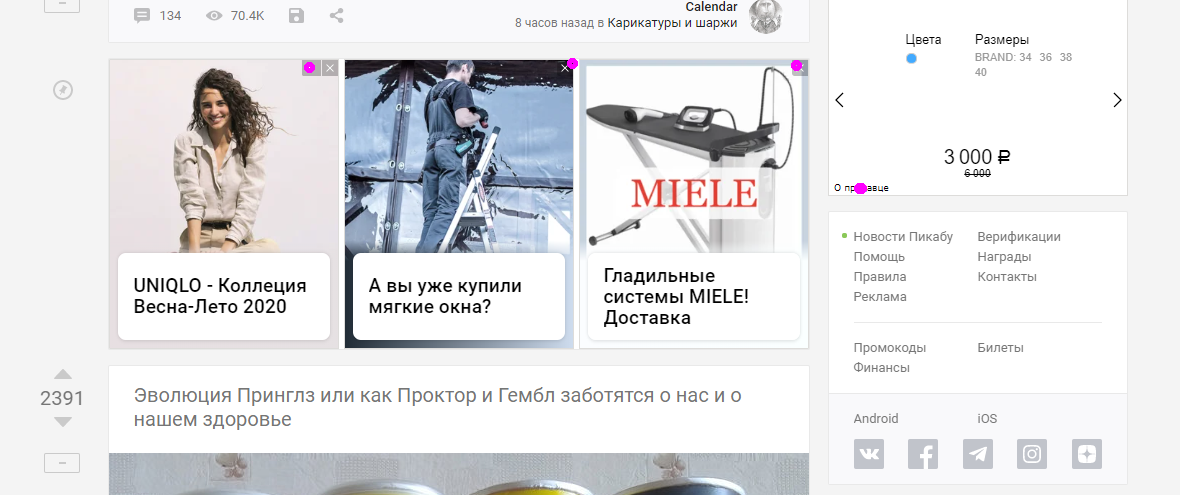
\includegraphics[scale=0.5]{violet_balls.PNG}
		\caption{Пример правильного корректного матчинга}
		\label{fig:violet_balls}
	\end{figure}
	
	\chapter{Приложение}
	

\section{Приложение A: ссылка на Github.}

\url{https://github.com/GhostKicker/imgproc\_coursework}
	
\end{document}


